\documentclass[../main.tex]{subfiles}
\graphicspath{{\subfix{../Figures/}}}

\begin{document}

\chapter{Methods}
\label{ch:methods}

We now present our work in more detail.
First, we discuss the specific problems we addressed and our proposed solutions.
Then, we introduce the datasets used in our experiments.

\section{Problem 0: CFX generation}

\subsection{Problem statement}

One possible formulation of the CFX generation problem is as follows:
\begin{quote}
Let $f: \R^\inputdim \to [0, 1]$ be a binary classifier such that $f(x)$ outputs the predicted probability of $x$ being in class 1.
Let $x$ be a point that is predicted to be of class 0, \ie{} such that $f(x) < \frac{1}{2}$.
Find a point $\CF{x}$ for which $f(\CF{x}) > \frac{1}{2}$ such that $\CF{x}$ is comparable with $x$ by a human.
\end{quote}

One solution to this is \ls{}.

\subsection{Proposed solutions}
\label{methods:0_sols}

\ls{} was presented by \citeauthor{cohenGifsplanation2022} in 2022 as a CF generation method for binary classification models on image data, specifically X-ray images of human lungs \cite{cohenGifsplanation2022}.
Given an input image $x$ predicted as class 0 (\ie{} for which $f(x)$ is low), \ls{} produces a new image close to $x$ that is predicted as class 1 (\ie{} for which $f(x)$ is high.).

In short, this is the method.
Let there be an autoencoder with $E$ the encoder and $D$ the decoder, and $z = E(x)$.
Then, given some coefficient $\lambda_\text{LS}$, a candidate counterfactual $x'$ is computed as:
\begin{align*}
    x' = D \left( z + \lambda_\text{LS} \grad{f(D(z))}{z} \right)
\end{align*}

In other words, $x$ is perturbed in the direction of the gradient of the classifier $f$ (the direction of steepest ascent), in order for $f$ to increase.
However, instead of computing the gradient in input space, they compute the gradient of the classifier \emph{in latent space} to promote realistic images.
Indeed, as discussed in \autoref{intro/image_data}, for many image problems the data can be assumed to lie on a low-dimensional subspace of $\inputspace$; therefore, if a generative model can recover this subspace, it can encode the input data in fewer dimensions with little information loss.

A summary diagram of the \ls{} procedure is shown in \autoref{fig:latent_shift}.
On the left, the data manifold in input space is non-convex, so by perturbing along the gradient in the input space we risk exiting the data manifold.
Hence, we first run the encoder, which we denote by $\enc$, then perturb the latent following the gradient of the classifier by some factor $\lambda_\text{LS}$, and finally run the decoder written $\dec$ to get the candidate counterfactual $\CF{x}$.

\begin{figure}[htbp]
	\centering
\subfile{../Figures/04_latent_shift.tex}
	\caption{A sketch of the \ls{} algorithm. Step 1 is applying $\enc$, step 2 is perturbing along the gradient of the classifier, and step 3 is applying $\dec$. Adapted from \cite{cohenGifsplanation2022}.}
	\label{fig:latent_shift}
\end{figure}

We outline some of the benefits of \ls{} here:

\begin{enumerate}
	\item First, this method is generally simple and easy to implement compared to some of those discussed in \autoref{ch:previous_work}.
	      It is also fast to perform once the generative model is trained, as it requires only one gradient computation (compared to an undetermined number in classical gradient-descent based solutions).

	\item Yet, one very interesting aspect of this method is that we can easily visualize the equivalent continuous path taken in input space (outlined in the left part of \autoref{fig:latent_shift}) by running the procedure with different values of $\lambda_\text{LS}$; thus we can see the final result $\CF{x}$, but also the full progression leading to it.
	      This is relevant for the problem of recourse mentioned in \autoref{par:cfx}: if a CFX is meant as advice for a data subject to alter their behavior to achieve a better outcome, then this advice would be more meaningful if the CFX would detail what \emph{individual steps} are needed to achieve that change.
	      This is outlined in research challenge no.~2 of \cite{vermaCounterfactual2020}.

	\item Finally, like in usual gradient descent, by setting $\lambda_\text{LS}$ to a negative value we can also produce new points that are \emph{more strongly} predicted as class 0.
\end{enumerate}

However, in the original \ls{} work, the method is applied to images, and the generative model used is an autoencoder architecture based on residual networks \cite{heDeep2015}.
This is an acceptable choice of model to image data, but it has two important consequences:
\begin{enumerate}
	\item The reconstruction error of the autoencoder is non-zero: encoding an image to get the starting point of the path is not an invertible operation.
	      This implies the CF path in input space generally does not go through the original point, even for $\lambda_\text{LS} = 0$; in fact, if the reconstruction error is too large this problem will impact the trustworthiness of the explanation.

	\item Basic autoencoders have no requirement to map inputs \emph{continuously}, so the generated path can look very complex which also makes the explanation less trustworthy.
\end{enumerate}

To overcome these issues, we turn to normalizing flows: generative models that are invertible by design.
Our analyses are generally not specific to normalizing flows though, so in the following we refer to our generative model as an autoencoder or a normalizing flow interchangeably.

We choose the NICE architecture from \cite{dinhNICE2015} presented in \autoref{bg/nf}.
In particular, we assume a standard Gaussian prior distribution, \ie{} we enforce that the distribution in the latent space is standard Gaussian.
As shown in \autoref{bg/nf}, for a Gaussian prior the $\nll$ is written:
\begin{align*}
\nll(x) = \frac{\latentdim}{2} \log 2 \pi
    +  \frac{z^T z}{2}
    - \sum_{i=1}^\latentdim \log \abs{S_{ii}}
\end{align*}
which is the loss that is minimized.

Importantly, there is nothing in our approach that cannot be done with the usual gradient descent procedure --
which has enjoyed many improvements to promote fast convergence and avoiding local minima \cite{kingmaAdam2014}.
The \ls{} method is nothing but a simplification of \revise{}, the procedure outlined in \cite{joshiRealistic2019},
where the gradient is computed only once and the constraint on the $L_1$ distance is dropped.
However, they differ in goals in that the authors of \cite{joshiRealistic2019} do not keep a record of the individual
steps taken during the gradient descent run.
Therefore, in the following we test our methods both on \ls{} and \revise{}, with and without the distance constraint
to stay close to the original \revise{} procedure.
Our objective is to study to what extent \ls{} can be used as a faster, perhaps less accurate CFX method.

\section{Problem 1: Multi-class extension}

\subsection{Problem statement}

Recall that the authors of \ls{} propose to recover a potential counterfactual by perturbing the input using the gradient of the classifier in latent space:
\begin{equation*}
    \CF{x} = \dec(z + \lambda_\text{LS} \nabla_z f(\dec(z))).
\end{equation*}

When $f$ is a binary classifier outputting the predicted probability that $x$ is of class 1, this is clearly sufficient.
However, in multi-class problems where $f$ outputs a vector in $\R^\outputdim$ there are several other functions we can use.
To see this, we reformulate the latent shift strategy with a generic loss that accounts for validity, denoted by $\lossval$:

Let $f$ be the classifier of interest, which outputs logits in $\R^\outputdim$ rather than a probability mass.
Given $x \in \inputspace$ and an autoencoder $\autoencoder = (\enc, \dec)$, a counterfactual path can be generated by computing the gradient of a so-called ``validity loss'' $\lossval$ and perturbing $z = \enc(x)$ in the direction of steepest \emph{descent} of $\lossval$:
\begin{equation*}
\CF{x} = \dec(z - \lambda \nabla_z \lossval(z)).
\end{equation*}

In vanilla \ls{}, the validity loss would then be $\lossval(z) = - \sigma(f(\dec(z)))$ where $\sigma$ denotes the sigmoid function, or any other increasing differentiable function that outputs a number in $[0, 1]$.

Hence, our problem is as follows:
\begin{quote}
Find a validity loss $\lossval$ that, for a given $x \in \inputspace$, gives rise to a class-changing path in input space when used in a gradient-based path generation method such as the one described above.
\end{quote}

\subsection{Proposed solutions}
\label{sec:validity_losses}

Note that this extension to the multi-class setting means that we have a choice to specify a given target class: we could set a requirement to simply change the class, without preference of target class.
In our analysis we focus on the case where a target class is specified.

In order to mimic the solution discussed in \cite{cohenGifsplanation2022}, we have
\begin{equation}
    \lossval(z) = -\softmax(f(\dec(z)))_\target,
\end{equation}
\ie{} the component of the output probability mass corresponding to class $\target$.
We call this loss $\PrbTarget$.
As before, the codomain is $[0, 1]$, and the loss corresponds directly to what we wish to achieve.
However, the multi-class setting assumption gives rise to other candidate losses.

Indeed, in the binary classification case, reaching towards the target class is exactly the same as moving away from the source class, since $p_\source = 1 - p_\target$.
By contrast, in the multi-class setting, different priorities need to be distinguished on a case-by-case basis: is it more important to reach the target (at the risk of potentially staying in the source class) or to get away from the source (at the risk of not reaching the target)?
The natural extension we presented is favoring the first option, but in fact there is no reason to neglect the second.

Thus, we introduce the following alternative loss, with regularization $\lambda \in [0, 1]$:
\begin{equation}
    \lossval(z) = -\softmax(f(\dec(z)))_\target
+ \lambda \softmax(f(\dec(z)))_\source
\end{equation}
which can be interpreted as adding the constraint of going towards the target as well as \emph{going away from the source}.
We call it $\PrbSource{\lambda}$.

In fact, we can go further:
in \ls{}, the objective of increasing $p_\target$ is also equivalent to decreasing $\mysum{c} p_c$, since in binary classification this is just $p_\source$; however, in multi-class problems they are distinct quantities.
Therefore we also define:
\begin{align*}
    \PrbOthers{\lambda}(z) = - \softmax(f(\dec(z)))_\target + \lambda \mysum{c} \softmax(f(\dec(z)))_c
\end{align*}
But notice
\begin{align*}
    \PrbOthers{\lambda}(z)
     & = - \softmax(f(\dec(z)))_\target + \lambda (1 - \softmax(f(\dec(z)))_\target) \\
     & = -(\lambda + 1) \softmax(f(\dec(z)))_\target + \lambda \\
     & = (\lambda + 1) \PrbTarget(z) + \lambda
\end{align*}
which is a rescaling of $\PrbTarget$, so in practice $\PrbOthers{}$ is not used.

To examine our intuition for why these proposals are sensible, we can compute the gradient of the loss, for example
\begin{align*}
\grad{\PrbSource{\lambda}}{z}
=  \grad{}{z} \left( - \softmax(f(\dec(z)))_\target + \lambda \softmax(f(\dec(z)))_\source \right)
\end{align*}

Because $z$ will only ever appear within $f(\dec(z))$, let $u = f(\dec(z))$ denote the output logits.
By the chain rule we have $\grad{\lossval}{z} = \grad{\lossval}{u} \grad{u}{z}$.
Furthermore, to lighten the calculations we let $p_i = \softmax(u)_i$ in what follows.

$\grad{u}{z}$ does not change with the loss so we focus on $\grad{\PrbSource{\lambda}}{u}$:
\begin{align*}
\grad{\PrbSource{\lambda}}{u}
=  \grad{}{u} \left( - p_\target + \lambda p_\source \right)
\end{align*}

We show in \autoref{eq:grad_softmax} that $\grad{p_i}{u_j} = p_i ( \dij  -  p_j)$ with $\dij$ the Kronecker delta.
Thus, the gradient of the loss is written:
\begin{align*}
    \grad{\lossval}{u_j}
=  - & \grad{p_\target }{u_j} + \lambda \grad{p_\source}{u_j}  \\
=  - & p_\target (\djt - p_j) + \lambda p_\source (\djs - p_j)
\end{align*}

Intuitively, a good validity loss should fulfill some basic requirements:
\begin{itemize}
\item When $p_\target$ is 1, we expect the gradient $\grad{\lossval}{z}$ to be close to 0; indeed, if the target is reached, there is no reason to keep perturbing $x$.
\item When $p_\target$ is 0, we expect the gradient $\grad{\lossval}{u}$ to be lower in the component corresponding to $\target$, so that the opposite of the gradient is higher in that component, which indicates the path is pushed towards $\target$.
\end{itemize}

Let us now examine whether these requirements are satisfied:
\begin{itemize}
    \item When $p_\target$ is 1, this means $p_j = \djt$, so we have for all $j$:
          \begin{align*}
                \grad{\PrbSource{\lambda}}{u_j} \\
                &= -1 \times (\djt -\djt) + \lambda \times 0 \times (\djs - p_j) \\
                &= 0\text{, as required.}
          \end{align*}
    \item When $p_\target$ is 0, we get:
          \begin{align*}
\grad{\PrbSource{\lambda}}{u_j}
& = -0 + \lambda p_\source (\djs - p_j)                        \\
               & = \begin{cases}
                       0                         & \text{if } j = \target \\
\lambda p_\source (1 - p_\source) & \text{if } j = \source \\
- \lambda p_\source p_j           & \text{otherwise}
                   \end{cases}
          \end{align*}
          The components for the classes that are not $\source$ or $\target$ are negative, which means these classes are favored compared to $\target$;
          this goes against our intuition.
\end{itemize}

Compare this with $\PrbTarget$: since $\PrbTarget = \PrbSource{\lambda=0}$ we see that in both cases $\grad{\PrbTarget}{u} = 0$.
This means that if the path gets stuck at $p_\target = 0$ then it cannot recover.

\subsubsection{Log-probability-based losses}

Setting the probability as an objective goes counter to the usual loss functions for training classifiers; a more common choice
for comparing predicted probabilities with true labels is the cross-entropy $\ce$ \cite{murphyMachine2012}.
The cross-entropy involves the logarithm of the predicted probabilities, so we can easily modify our previous attempts to get:
\begin{align*}
    \LogPrbTarget{}:        & \quad    \lossval(u) = - \log p_\target                              \\
    \LogPrbSource{\lambda}: & \quad     \lossval(u) = - \log p_\target + \lambda \log p_\source    \\
    \LogPrbOthers{\lambda}: & \quad    \lossval(u) = - \log p_\target + \lambda \mysum{c} \log p_c
\end{align*}
where $\lambda \in [0, 1]$ is a regularization parameter.

Let us compute the gradients of our log-probability losses to get a better understanding of their behavior.

We have
\begin{align*}
    \grad{\log p_i}{u_j}
= \grad{p_i}{u_j} / p_i
= \frac{p_i (\dij - p_j) }{p_i}
= \dij - p_j
\end{align*}
Hence
\begin{align*}
    \grad{\LogPrbSource{\lambda}}{u_j}
     & = - \grad{\log p_\target}{u_j} + \lambda \grad{\log p_\source}{u_j} \\
     & = - (\djt - p_j) + \lambda (\djs - p_j)                             \\
     & = - \djt + p_j + \lambda \djs - \lambda p_j                         \\
     & = (1 - \lambda) p_j + \lambda \djs - \djt.
\end{align*}
We check our intuition:
\begin{itemize}
    \item For $p_\target = 1$ this gives us
          \begin{align*}
              \grad{\LogPrbSource{\lambda}}{u_j}
               & = (1 - \lambda) \djt + \lambda \djs - \djt \\
               & = \lambda(\djs - \djt)                     \\
               & = \begin{cases}
                       -\lambda & \text{if } j = \target \\
                       \lambda  & \text{if } j = \source \\
                       0        & \text{otherwise,}
                   \end{cases}
          \end{align*}
          so the gradient keeps pushing $u_\target$ higher and $u_\source$ lower, as required.
          When $\lambda = 0$, which corresponds to $\LogPrbTarget$, the gradient is zero which is also acceptable intuitively.

    \item For $p_\target = 0$ we get
          \begin{align*}
              \grad{\LogPrbSource{\lambda}}{u_j}
               & = (1 - \lambda) p_j + \lambda \djs - \djt                 \\
               & = \begin{cases}
                       -1                             & \text{if } j = \target \\
                       (1-\lambda)p_\source + \lambda & \text{if } j = \source \\
                       (1 - \lambda) p_j              & \text{otherwise.}
                   \end{cases}
          \end{align*}
          When $j \neq \target$ the gradient is larger than 0 so again, class $\target$ dominates.
\end{itemize}

For $\LogPrbOthers{}$ we have:
\begin{align*}
    \grad{\LogPrbOthers{\lambda}}{u_j}
     = p_j (1 - \lambda (\outputdim - 1)) + \lambda (1 - \djt) - \djt.
\end{align*}
The full derivation can be found in \autoref{eq:grad_log_prb_others}.

We check our intuition:
\begin{itemize}
    \item For $p_\target = 1$ this gives us
          \begin{align*}
              \grad{\LogPrbOthers{\lambda}}{u_j}
               & = \djt (1 - \lambda (\outputdim - 1)) + \lambda (1 - \djt) - \djt      \\
               & = \djt - \djt \lambda (\outputdim - 1) + \lambda - \lambda \djt - \djt \\
               & = - \djt \lambda (\outputdim - 1) + \lambda - \lambda \djt             \\
               & = - \lambda (\djt (\outputdim - 1) - 1 + \djt)                         \\
               & = - \lambda (\outputdim \djt - 1)                                      \\
               & = \begin{cases}
                       - (\outputdim - 1) \lambda & \text{if } j = \target \\
                       \lambda                    & \text{otherwise}
                   \end{cases}
          \end{align*}
          so the gradient pushes $u_\target$ higher than that for other classes, as required.

    \item For $p_\target = 0$ we get
          \begin{align*}
              \grad{\LogPrbOthers{\lambda}}{u_j}
               & = p_j (1 - \lambda (\outputdim - 1)) + \lambda (1 - \djt) - \djt        \\
               & = \begin{cases}
                       -1                                           & \text{if } j = \target \\
                       p_j(1 - \lambda ( \outputdim -1 )) + \lambda & \text{otherwise}
                   \end{cases}
          \end{align*}
Here it is unclear if $u_j$ is more negative than $-1$.
It turns out it can be: for example, if $\lambda = 1$ and $p_j = 1$ then we get $1 - (\outputdim -1) + 1 = 3 - \outputdim$, so for $\outputdim > 4$, $u_j$ will be pushed higher than $u_\target$.
\end{itemize}


\subsubsection{Logit-based losses}

Our previous loss functions are somewhat difficult to control because of the interactions between the different classes:
when we state our requirement to increase $p_\target$, this can be understood either as increasing $u_\target$, or as decreasing the other $u_c$.
For this reason, we formulate losses optimizing for the logits directly (with $\lambda \in [0, 1]$):
\begin{align*}
    \LogitTarget{}:        & \quad    \lossval(u) = - u_\target                         \\
    \LogitSource{\lambda}: & \quad     \lossval(u) = - u_\target + \lambda u_\source    \\
    \LogitOthers{\lambda}: & \quad    \lossval(u) = - u_\target + \lambda \mysum{c} u_c
\end{align*}

Here the gradients are easy to compute since the loss is linear in the logits:
\begin{align*}
\grad{\LogitTarget{}}{u_j} &= - \djt                         \\
\grad{\LogitSource{\lambda}}{u_j} &= - \djt + \lambda \djs                        \\
\grad{\LogitOthers{\lambda}}{u_j}
&= - \djt + \lambda \mysum{c} \delta_{jc} \\
&= - \djt + \lambda \times \begin{cases}
    0 & \text{if } j = \target \\
    1 & \text{otherwise} 
\end{cases} \\
&= - \djt + \lambda (1 - \djt) \\
&= -(\lambda + 1)\djt + \lambda.
\end{align*}
Hence the behavior is also clear: in all cases $u_\target$ always gets pushed up higher than the other logits, no matter the value of $u$.



\section{Problem 2: Path regularization}

\subsection{Problem statement}

In this section and in the following, we denote a CFX path by $(x_t)_{t=1}^T \in \inputspace^T$, where $x_T$ is the end point of the path and
$x_1$ is its starting point, ideally as close to $x$ as possible.
Similarly, we also define $(z_t)_{t=1}^T \in \latentspace^T$ such that $(x_t)_{t=1}^T = (\dec(z_t))_{t=1}^T$.

A typical requirement on a counterfactual $\CF{x}$ for an input $x$ is for $\norm{\CF{x} - x}$ to be small, where $\norm{\cdot}$ is the $L_1$ norm for example.
While this makes sense for methods that produce a discrete set of counterfactuals, we focus on methods that produce \emph{continuous explanation paths}, hence we wish to ensure these requirements are satisfied \emph{along the path}.
In the example of distance, this would give us the constraint that the endpoint of the path $\CF{x} = \dec(z_T)$ be close to the starting point, but also that \emph{on the whole} the path $(z_t)_{t=1}^T$ stay as close as possible to the starting point.

In the case of gradient-descent optimization paths, this can be addressed by placing these constraints in the loss function during the computation of the next step: this is done in \revise{}, where the loss function includes the $L_1$ distance \cite{joshiRealistic2019}:
\begin{equation*}
\cfloss(z_t) = \lossval(z_t) + \lambda_\text{distance} \norm{\dec(z_t) - x}_1.
\end{equation*}
However, for \ls{} this solution is not appropriate because the gradient is only computed \emph{once}, for $z = \enc(x)$.
Indeed, even though the first step goes in the right direction, overall the whole path can still go in the wrong direction because the information carried by the gradient is less relevant the further away we go from the input.

Hence, our second problem statement is the following:
\begin{quote}
Given a path CF method which may or may not produce paths using an iterative procedure, but which involves a generative model such as a normalizing flow,
how can we constrain a whole path $(x_t)_{t=1}^T$ according to some requirements?
\end{quote}

\subsection{Proposed solution}

Since we can extend many of the point-wise measures to whole paths in a natural way, \eg{} with the mean or the maximum, we propose applying this as a loss on the whole path and using it to \emph{train the autoencoder} in addition to its usual loss function (\eg{} the $\nll$).
This added component to the loss can take various forms, and in general we call it \emph{path regularization}.
The full process is described with pseudocode in \autoref{algo:pathreg}.
Note that in NF-based autoencoders, the decoder is the inverse of the encoder and thus does not need to be trained like it would in a VAE; this is why we show explicitly only the trainable parameters of $\enc$ (denoted by $\phi$).

\begin{algorithm}
\caption{Learning a normalizing flow latent space by SGD with path regularization}
\label{algo:pathreg}
\KwData{Classifier $f, \autoencoder\ (\enc_\phi, \dec),$ (training) data, CF loss $\cfloss$, path loss $\pathloss$, path loss regularization coefficient $\lambda_\apath$}
\KwOut{$\phi^*$ that minimizes the $\nll$ and the path loss}
\While{not converged}{
$x \gets \mathtt{get\_input}(\text{data})$ \\
$z \gets \enc_\phi(x)$ \\
$\source \gets \arg\max_{c \in \setclasses} f(x)$ \\
$\target \gets \mathtt{random\_target}(x)$ \tcp*{such that $\target \neq \source$}
$\apath \gets \mathtt{generate\_path}_{\cfloss}(z, \source, \target)$ \tcp*{$\apath = (\CF{x}_t)_{t=1}^T$}
$\phi \gets \phi - \nabla_\phi {(\nll(z) + \lambda_\apath \pathloss(\apath) + \lambda_\text{CF} \cfloss(\apath))}$ \\
}
\end{algorithm}

Since the one obvious constraint on paths is that they should be valid, we include a term $\cfloss$ which would typically be an average over the path of whatever loss was used to compute the path, which should include some constraints on validity; this is what we do in our analyses.
\note{I ended up not using this in the end; what do i do?}

$\pathloss$ represents our criteria for an interpretable path. So what criteria should we enforce?
We choose to apply the following constraint: the path should go from $\source$ to $\target$ passing through as few other classes as possible, and ideally, without passing through any other class.
Thus we formulate $\BoundaryCrossLoss$ as follows:
\begin{align*}
\BoundaryCrossLoss(\apath) = -
\frac{1}{\nbsteps} \sum_{t=1}^{\nbsteps}
\max \{ p^{(t)}_\source, p^{(t)}_\target \}
\end{align*}
where $p^{(t)}_i$ is the predicted probability $\softmax(f(x_t))_i$.

Note that class information is indirectly given during the training of the autoencoder, so the autoencoder is dependent on the classification task.
By contrast, in vanilla \ls{} the authors make a conscious decision to keep the autoencoder entirely separate from the classifier.
Their justification is that this allows for reusing the autoencoder on classifiers that have learned different tasks but that act on the same input data; for example, different classifiers each trained to detect a particular lung disease.
While a valid argument, \citeauthor{locatelloChallenging2019} have demonstrated that some properties of latent representations can only be achieved in the presence of class label information \cite{locatelloChallenging2019}.

\section{Robustness of path regularization}
\label{methods:robustness}

\subsection{Problem statement}

The path regularization algorithm admits a general loss $\pathloss$ which is problem-dependent.
Yet, this raises a question: can the path regularization algorithm accommodate for any path loss, however exotic?
If so, this procedure can be manipulated to produce adversarial paths that do not reflect the true behavior of the explained model.

\subsection{Proposed experiment}

To probe the possibility of abuse of the path regularization procedure, we formulate an adversarial loss that promotes paths going through a specific point $\xgoal$:
\begin{align}
    \pathloss(\xgoal, (z_t)_{t=1}^T) = \min_{t \in \{1, \ldots, T\}} \{ \norm{\dec(z_t) - \xgoal}_2 \}
\end{align}
The goal of the experiment is to verify whether path regularized latent representations lead to paths that fit this
criterion while staying valid.

\section{Datasets}
\label{sec:datasets}

In our experiments we use one custom synthetic dataset generated in a parametrizable way, as well as some real datasets.

We always take out the categorical features and we standardize each feature.

\subsection{\CakeOnSea}

Our analyses are complicated by the impossibility of visualizing counterfactuals for tabular data in general.
Thus, in order to start approaching the problem intuitively, one of our datasets is a synthetic dataset with no more than two features having an influence on the response.
The two features, denoted by $x_0$ and $x_1$, range from 0 to 50, except for the so-called ``dead zone'' which is $[25, 35]^2$, in which there are no points at all.
There are three classes, and the class decision rule is as follows:
\begin{align*}
    (x_0, x_1) \in [35, 45]^2 \implies & y = 2 \\
    x_1 < 25                  \implies & y = 0 \\
    (x_0, x_1) \in \text{dead zone} \lor (x_0, x_1) \notin [0, 50]^2  \implies & y\ \text{unknown} \\
    \text{otherwise} \qquad            & y = 1
\end{align*}
Note that we explicitly refrain from assigning a class to points in the dead zone or outside $[0, 50]^2$.
The decision rule can be visualized in \autoref{fig:cake_on_sea}.

To generate the dataset, we randomly sample points in the $[0, 50]^2$ square and then take out points from the dead zone. By default, the sampling distribution is a uniform $\mathcal{U}([0, 50]^2)$.

Our implementation also allows for producing more features that are linear combinations of the first two, to simulate data with an arbitrary number of columns while keeping the dataset structure intact.
However, in the interest of keeping things simple, we use only the 2-feature version in our analyses.

\begin{figure}[h]
    \centering


\tikzset{every picture/.style={line width=0.75pt}} %set default line width to 0.75pt        

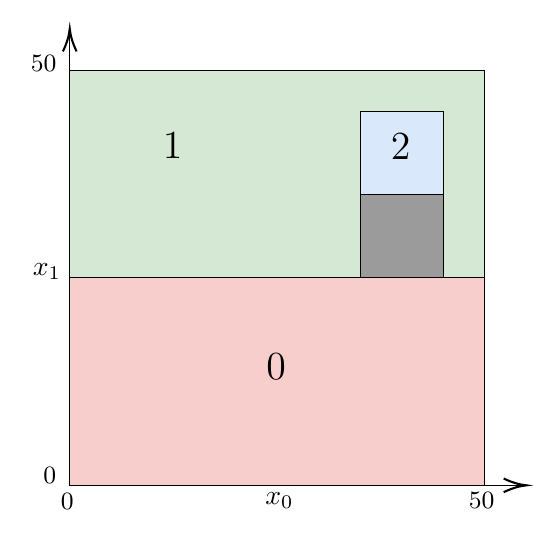
\begin{tikzpicture}[x=0.75pt,y=0.75pt,yscale=-1,xscale=1]
%uncomment if require: \path (0,300); %set diagram left start at 0, and has height of 300

%Shape: Rectangle [id:dp12943827359599314] 
\draw  [fill={rgb, 255:red, 213; green, 232; blue, 212 }  ,fill opacity=1 ] (250,50) -- (450,50) -- (450,150) -- (250,150) -- cycle ;
%Straight Lines [id:da8416607833401318] 
\draw    (250,250) -- (250,32) ;
\draw [shift={(250,30)}, rotate = 90] [color={rgb, 255:red, 0; green, 0; blue, 0 }  ][line width=0.75]    (10.93,-3.29) .. controls (6.95,-1.4) and (3.31,-0.3) .. (0,0) .. controls (3.31,0.3) and (6.95,1.4) .. (10.93,3.29)   ;
%Straight Lines [id:da5577600596159713] 
\draw    (250,250) -- (468,250) ;
\draw [shift={(470,250)}, rotate = 180] [color={rgb, 255:red, 0; green, 0; blue, 0 }  ][line width=0.75]    (10.93,-3.29) .. controls (6.95,-1.4) and (3.31,-0.3) .. (0,0) .. controls (3.31,0.3) and (6.95,1.4) .. (10.93,3.29)   ;
%Straight Lines [id:da17568384394881242] 
\draw    (250,150) -- (450,150) ;
%Shape: Rectangle [id:dp3705541448905584] 
\draw  [fill={rgb, 255:red, 248; green, 206; blue, 204 }  ,fill opacity=1 ] (250,150) -- (450,150) -- (450,250) -- (250,250) -- cycle ;
%Shape: Rectangle [id:dp5334639009219723] 
\draw  [fill={rgb, 255:red, 218; green, 232; blue, 252 }  ,fill opacity=1 ] (390,70) -- (430,70) -- (430,110) -- (390,110) -- cycle ;
%Shape: Rectangle [id:dp05533155300504711] 
\draw  [fill={rgb, 255:red, 155; green, 155; blue, 155 }  ,fill opacity=1 ] (390,110) -- (430,110) -- (430,150) -- (390,150) -- cycle ;

% Text Node
\draw (343.5,185.33) node [anchor=north west][inner sep=0.75pt]  [font=\Large]  {$0$};
% Text Node
\draw (293.6,79) node [anchor=north west][inner sep=0.75pt]  [font=\Large]  {$1$};
% Text Node
\draw (403.5,79.33) node [anchor=north west][inner sep=0.75pt]  [font=\Large]  {$2$};
% Text Node
\draw (343,252) node [anchor=north west][inner sep=0.75pt]    {$x_{0}$};
% Text Node
\draw (231,142) node [anchor=north west][inner sep=0.75pt]    {$x_{1}$};
% Text Node
\draw (244.5,252.67) node [anchor=north west][inner sep=0.75pt]  [font=\small]  {$0$};
% Text Node
\draw (236,240.33) node [anchor=north west][inner sep=0.75pt]  [font=\small]  {$0$};
% Text Node
\draw (230,41.67) node [anchor=north west][inner sep=0.75pt]  [font=\small]  {$50$};
% Text Node
\draw (441,252) node [anchor=north west][inner sep=0.75pt]  [font=\small]  {$50$};


\end{tikzpicture}

\caption{Decision rule for the \CakeOnSea dataset. The so-called ``dead zone'' is shown in dark gray between class 2 and class 0.}
    \label{fig:cake_on_sea}
\end{figure}

\subsection{\ForestCover}

This dataset is taken from the UCI Machine Learning repository\footnote{\url{https://archive.ics.uci.edu/ml/datasets/Covertype}} \cite{duaUCI2019} based on work in \cite{blackardComparative1999}.
It contains data on 581012 trees such as their elevation, their horizontal distance to the nearest surface water features and the type of soil they are in, as well as their species, among seven tree species. There is a total of 13 recorded variables, including the tree species. Of the 12 variables used for prediction, two are categorical, and encoded as one-hot columns.
Because our method does not trivially extend to categorical features yet, we remove the one-hot columns; we thus have $D = 10$.

\subsection{\WineQuality}

The \WineQuality{} dataset originates from \cite{cortezModeling2009} and can be found in the UCI repository\footnote{\url{https://archive.ics.uci.edu/ml/datasets/Wine+Quality}}.
It consists of data on 6498 Portuguese ``Vinho Verde'' wines, such as their pH, their density and their alcohol percentage, as well as a quality rating from 0 to 10.
There are 13 variables including the quality rating column; except for the quality and whether they are red or white, all of them are numerical.
As before, we remove the red/white information.

Because the wine quality is an ordinal variable (categorical but ordered), it is not necessarily appropriate to run a classifier on the dataset directly;
thus, we group quality ratings together into 3 classes.
In fact, there are no wines with a quality rating of 0, 1, 2 or 10, and 43\% of the rows have a rating of 6 out of 10.
Hence, for our classification task we create the following class mapping:
\begin{itemize}
    \item class 0 corresponds to a quality rating of 5 or lower (33\% of the data),
    \item class 1 to a rating of 6 (43\%) and
    \item class 2 to a rating of 7 or higher (18\%).
\end{itemize}

\subsection{\OnlineNewsPopularity}

This dataset \cite{fernandesProactive2015} also from the UCI repository\footnote{\url{https://archive.ics.uci.edu/ml/datasets/Online+News+Popularity}} contains data on 39644 news posts recovered from the Mashable website, such as the number of HTML tags of a certain type, the time of publishing, and also machine-learning-derived features such as the subjectivity and polarity of the language used, and how well the post fits within a given topic as determined by LDA.
As before, we remove the categorical columns, leaving us with 46 columns including the target variable.

The target variable is the number of shares of a given article, which is an integer; in order to make it usable for classification tasks, we create the following class mapping:
\begin{itemize}
    \item Articles with a number of shares below the median (\ie{} in the worst 50\%) are considered to be in class 0,
    \item Articles between the 50\% and the 75\% percentiles are considered class 1,
    \item Articles between the 75\% and 95\% percentiles are considered class 2,
\item Articles above the 95\% percentile (\ie{} in the best 5\%) are considered class 3.
\end{itemize}
Thus, class 0 contains 50\% of the data, class 1 contains 25\%, class 2 contains 20\% and class 3 contains 5\%.

\subsection{Summary of datasets}

All datasets are divided into training, validation, and test sets containing 60\%, 20\%, and 20\% of the data respectively.

In \autoref{tab:datasets} we summarize the relevant information about our datasets and settings when using them for training.

\begin{table}[h!]
    \centering
\begin{tabular}{lrrrrrr}
        \toprule
Name          & $\inputdim$ & $\outputdim$ & $\card{\trainset}$     & $\card{\valset}$     & $\card{\testset}$    & $
\card{\trainset} / \inputdim$  \\
        \midrule
\CakeOnSea            & 2           & 3            & 57607                  & 19202                & 19202        & 28803                    \\
\ForestCover          & 10          & 7            & 348608                 & 116202               & 116202       & 34861                   \\
\WineQuality          & 11          & 3            & 3900                   & 1299                 & 1299          & 355                  \\
\OnlineNewsPopularity & 45          & 4            & 23788                  & 7928                 & 7928          & 529                   \\
        \bottomrule
    \end{tabular}
    \caption{Summary of our dataset settings. $\inputdim$ refers to the number of features, $\outputdim$ to the number of classes, and $\abs{\trainset}$, $\abs{\valset}$, $\abs{\testset}$ to the size of the train, validation, and test set respectively.}
    \label{tab:datasets}
\end{table}

We are now in position to describe our experiments and findings.

\end{document}
